% Options for packages loaded elsewhere
\PassOptionsToPackage{unicode}{hyperref}
\PassOptionsToPackage{hyphens}{url}
%
\documentclass[
]{book}
\usepackage{lmodern}
\usepackage{amssymb,amsmath}
\usepackage{ifxetex,ifluatex}
\ifnum 0\ifxetex 1\fi\ifluatex 1\fi=0 % if pdftex
  \usepackage[T1]{fontenc}
  \usepackage[utf8]{inputenc}
  \usepackage{textcomp} % provide euro and other symbols
\else % if luatex or xetex
  \usepackage{unicode-math}
  \defaultfontfeatures{Scale=MatchLowercase}
  \defaultfontfeatures[\rmfamily]{Ligatures=TeX,Scale=1}
\fi
% Use upquote if available, for straight quotes in verbatim environments
\IfFileExists{upquote.sty}{\usepackage{upquote}}{}
\IfFileExists{microtype.sty}{% use microtype if available
  \usepackage[]{microtype}
  \UseMicrotypeSet[protrusion]{basicmath} % disable protrusion for tt fonts
}{}
\makeatletter
\@ifundefined{KOMAClassName}{% if non-KOMA class
  \IfFileExists{parskip.sty}{%
    \usepackage{parskip}
  }{% else
    \setlength{\parindent}{0pt}
    \setlength{\parskip}{6pt plus 2pt minus 1pt}}
}{% if KOMA class
  \KOMAoptions{parskip=half}}
\makeatother
\usepackage{xcolor}
\IfFileExists{xurl.sty}{\usepackage{xurl}}{} % add URL line breaks if available
\IfFileExists{bookmark.sty}{\usepackage{bookmark}}{\usepackage{hyperref}}
\hypersetup{
  pdftitle={A Minimal Book Example},
  pdfauthor={Brandon Stark},
  hidelinks,
  pdfcreator={LaTeX via pandoc}}
\urlstyle{same} % disable monospaced font for URLs
\usepackage{color}
\usepackage{fancyvrb}
\newcommand{\VerbBar}{|}
\newcommand{\VERB}{\Verb[commandchars=\\\{\}]}
\DefineVerbatimEnvironment{Highlighting}{Verbatim}{commandchars=\\\{\}}
% Add ',fontsize=\small' for more characters per line
\usepackage{framed}
\definecolor{shadecolor}{RGB}{248,248,248}
\newenvironment{Shaded}{\begin{snugshade}}{\end{snugshade}}
\newcommand{\AlertTok}[1]{\textcolor[rgb]{0.94,0.16,0.16}{#1}}
\newcommand{\AnnotationTok}[1]{\textcolor[rgb]{0.56,0.35,0.01}{\textbf{\textit{#1}}}}
\newcommand{\AttributeTok}[1]{\textcolor[rgb]{0.77,0.63,0.00}{#1}}
\newcommand{\BaseNTok}[1]{\textcolor[rgb]{0.00,0.00,0.81}{#1}}
\newcommand{\BuiltInTok}[1]{#1}
\newcommand{\CharTok}[1]{\textcolor[rgb]{0.31,0.60,0.02}{#1}}
\newcommand{\CommentTok}[1]{\textcolor[rgb]{0.56,0.35,0.01}{\textit{#1}}}
\newcommand{\CommentVarTok}[1]{\textcolor[rgb]{0.56,0.35,0.01}{\textbf{\textit{#1}}}}
\newcommand{\ConstantTok}[1]{\textcolor[rgb]{0.00,0.00,0.00}{#1}}
\newcommand{\ControlFlowTok}[1]{\textcolor[rgb]{0.13,0.29,0.53}{\textbf{#1}}}
\newcommand{\DataTypeTok}[1]{\textcolor[rgb]{0.13,0.29,0.53}{#1}}
\newcommand{\DecValTok}[1]{\textcolor[rgb]{0.00,0.00,0.81}{#1}}
\newcommand{\DocumentationTok}[1]{\textcolor[rgb]{0.56,0.35,0.01}{\textbf{\textit{#1}}}}
\newcommand{\ErrorTok}[1]{\textcolor[rgb]{0.64,0.00,0.00}{\textbf{#1}}}
\newcommand{\ExtensionTok}[1]{#1}
\newcommand{\FloatTok}[1]{\textcolor[rgb]{0.00,0.00,0.81}{#1}}
\newcommand{\FunctionTok}[1]{\textcolor[rgb]{0.00,0.00,0.00}{#1}}
\newcommand{\ImportTok}[1]{#1}
\newcommand{\InformationTok}[1]{\textcolor[rgb]{0.56,0.35,0.01}{\textbf{\textit{#1}}}}
\newcommand{\KeywordTok}[1]{\textcolor[rgb]{0.13,0.29,0.53}{\textbf{#1}}}
\newcommand{\NormalTok}[1]{#1}
\newcommand{\OperatorTok}[1]{\textcolor[rgb]{0.81,0.36,0.00}{\textbf{#1}}}
\newcommand{\OtherTok}[1]{\textcolor[rgb]{0.56,0.35,0.01}{#1}}
\newcommand{\PreprocessorTok}[1]{\textcolor[rgb]{0.56,0.35,0.01}{\textit{#1}}}
\newcommand{\RegionMarkerTok}[1]{#1}
\newcommand{\SpecialCharTok}[1]{\textcolor[rgb]{0.00,0.00,0.00}{#1}}
\newcommand{\SpecialStringTok}[1]{\textcolor[rgb]{0.31,0.60,0.02}{#1}}
\newcommand{\StringTok}[1]{\textcolor[rgb]{0.31,0.60,0.02}{#1}}
\newcommand{\VariableTok}[1]{\textcolor[rgb]{0.00,0.00,0.00}{#1}}
\newcommand{\VerbatimStringTok}[1]{\textcolor[rgb]{0.31,0.60,0.02}{#1}}
\newcommand{\WarningTok}[1]{\textcolor[rgb]{0.56,0.35,0.01}{\textbf{\textit{#1}}}}
\usepackage{longtable,booktabs}
% Correct order of tables after \paragraph or \subparagraph
\usepackage{etoolbox}
\makeatletter
\patchcmd\longtable{\par}{\if@noskipsec\mbox{}\fi\par}{}{}
\makeatother
% Allow footnotes in longtable head/foot
\IfFileExists{footnotehyper.sty}{\usepackage{footnotehyper}}{\usepackage{footnote}}
\makesavenoteenv{longtable}
\usepackage{graphicx,grffile}
\makeatletter
\def\maxwidth{\ifdim\Gin@nat@width>\linewidth\linewidth\else\Gin@nat@width\fi}
\def\maxheight{\ifdim\Gin@nat@height>\textheight\textheight\else\Gin@nat@height\fi}
\makeatother
% Scale images if necessary, so that they will not overflow the page
% margins by default, and it is still possible to overwrite the defaults
% using explicit options in \includegraphics[width, height, ...]{}
\setkeys{Gin}{width=\maxwidth,height=\maxheight,keepaspectratio}
% Set default figure placement to htbp
\makeatletter
\def\fps@figure{htbp}
\makeatother
\setlength{\emergencystretch}{3em} % prevent overfull lines
\providecommand{\tightlist}{%
  \setlength{\itemsep}{0pt}\setlength{\parskip}{0pt}}
\setcounter{secnumdepth}{5}
\usepackage{booktabs}
\usepackage[margin=1in]{geometry}
\usepackage[]{natbib}
\bibliographystyle{apalike}

\title{A Minimal Book Example}
\author{Brandon Stark}
\date{2021-01-28}

\usepackage{amsthm}
\newtheorem{theorem}{Theorem}[chapter]
\newtheorem{lemma}{Lemma}[chapter]
\newtheorem{corollary}{Corollary}[chapter]
\newtheorem{proposition}{Proposition}[chapter]
\newtheorem{conjecture}{Conjecture}[chapter]
\theoremstyle{definition}
\newtheorem{definition}{Definition}[chapter]
\theoremstyle{definition}
\newtheorem{example}{Example}[chapter]
\theoremstyle{definition}
\newtheorem{exercise}{Exercise}[chapter]
\theoremstyle{remark}
\newtheorem*{remark}{Remark}
\newtheorem*{solution}{Solution}
\begin{document}
\maketitle

{
\setcounter{tocdepth}{1}
\tableofcontents
}
\hypertarget{prerequisites}{%
\chapter{Prerequisites}\label{prerequisites}}

This is a \emph{sample} book written in \textbf{Markdown}. You can use anything that Pandoc's Markdown supports, e.g., a math equation \(a^2 + b^2 = c^2\).

The \textbf{bookdown} package can be installed from CRAN or Github:

\begin{Shaded}
\begin{Highlighting}[]
\KeywordTok{install.packages}\NormalTok{(}\StringTok{"bookdown"}\NormalTok{)}
\CommentTok{# or the development version}
\CommentTok{# devtools::install_github("rstudio/bookdown")}
\end{Highlighting}
\end{Shaded}

Remember each Rmd file contains one and only one chapter, and a chapter is defined by the first-level heading \texttt{\#}.

To compile this example to PDF, you need XeLaTeX. You are recommended to install TinyTeX (which includes XeLaTeX): \url{https://yihui.org/tinytex/}.

\hypertarget{intro}{%
\chapter{Introduction}\label{intro}}

You can label chapter and section titles using \texttt{\{\#label\}} after them, e.g., we can reference Chapter \ref{intro}. If you do not manually label them, there will be automatic labels anyway, e.g., Chapter \ref{root-locus}.

Figures and tables with captions will be placed in \texttt{figure} and \texttt{table} environments, respectively.

\begin{Shaded}
\begin{Highlighting}[]
\KeywordTok{par}\NormalTok{(}\DataTypeTok{mar =} \KeywordTok{c}\NormalTok{(}\DecValTok{4}\NormalTok{, }\DecValTok{4}\NormalTok{, }\FloatTok{.1}\NormalTok{, }\FloatTok{.1}\NormalTok{))}
\KeywordTok{plot}\NormalTok{(pressure, }\DataTypeTok{type =} \StringTok{'b'}\NormalTok{, }\DataTypeTok{pch =} \DecValTok{19}\NormalTok{)}
\end{Highlighting}
\end{Shaded}

\begin{figure}

{\centering 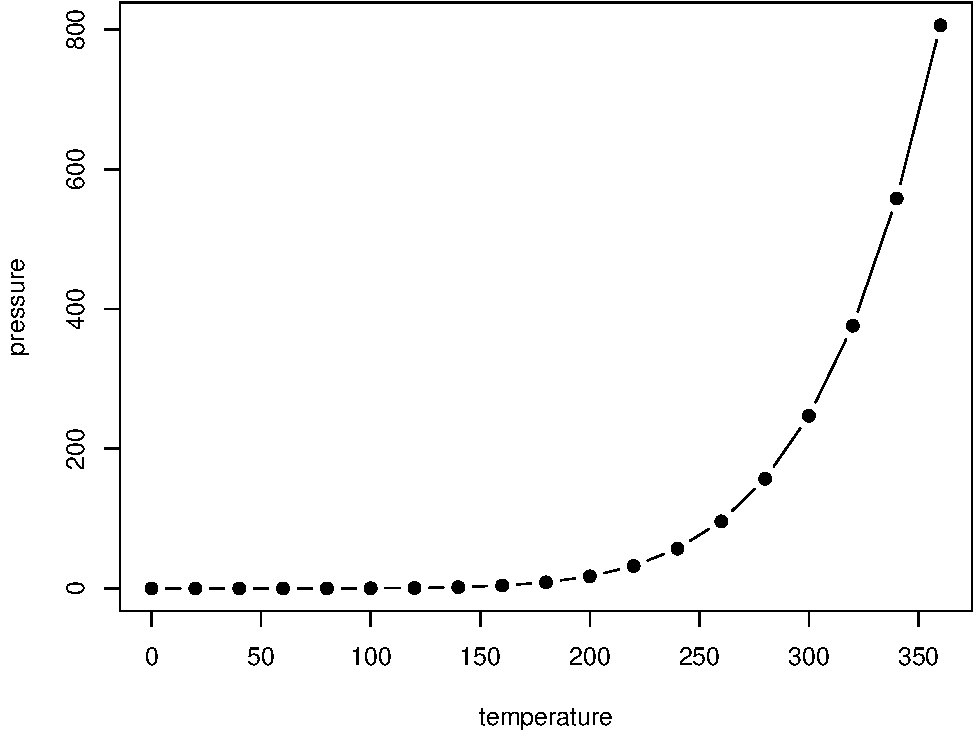
\includegraphics[width=0.8\linewidth]{stunning-chainsaw_files/figure-latex/nice-fig-1} 

}

\caption{Here is a nice figure!}\label{fig:nice-fig}
\end{figure}

Reference a figure by its code chunk label with the \texttt{fig:} prefix, e.g., see Figure \ref{fig:nice-fig}. Similarly, you can reference tables generated from \texttt{knitr::kable()}, e.g., see Table \ref{tab:nice-tab}.

\begin{Shaded}
\begin{Highlighting}[]
\NormalTok{knitr}\OperatorTok{::}\KeywordTok{kable}\NormalTok{(}
  \KeywordTok{head}\NormalTok{(iris, }\DecValTok{20}\NormalTok{), }\DataTypeTok{caption =} \StringTok{'Here is a nice table!'}\NormalTok{,}
  \DataTypeTok{booktabs =} \OtherTok{TRUE}
\NormalTok{)}
\end{Highlighting}
\end{Shaded}

\begin{table}

\caption{\label{tab:nice-tab}Here is a nice table!}
\centering
\begin{tabular}[t]{rrrrl}
\toprule
Sepal.Length & Sepal.Width & Petal.Length & Petal.Width & Species\\
\midrule
5.1 & 3.5 & 1.4 & 0.2 & setosa\\
4.9 & 3.0 & 1.4 & 0.2 & setosa\\
4.7 & 3.2 & 1.3 & 0.2 & setosa\\
4.6 & 3.1 & 1.5 & 0.2 & setosa\\
5.0 & 3.6 & 1.4 & 0.2 & setosa\\
\addlinespace
5.4 & 3.9 & 1.7 & 0.4 & setosa\\
4.6 & 3.4 & 1.4 & 0.3 & setosa\\
5.0 & 3.4 & 1.5 & 0.2 & setosa\\
4.4 & 2.9 & 1.4 & 0.2 & setosa\\
4.9 & 3.1 & 1.5 & 0.1 & setosa\\
\addlinespace
5.4 & 3.7 & 1.5 & 0.2 & setosa\\
4.8 & 3.4 & 1.6 & 0.2 & setosa\\
4.8 & 3.0 & 1.4 & 0.1 & setosa\\
4.3 & 3.0 & 1.1 & 0.1 & setosa\\
5.8 & 4.0 & 1.2 & 0.2 & setosa\\
\addlinespace
5.7 & 4.4 & 1.5 & 0.4 & setosa\\
5.4 & 3.9 & 1.3 & 0.4 & setosa\\
5.1 & 3.5 & 1.4 & 0.3 & setosa\\
5.7 & 3.8 & 1.7 & 0.3 & setosa\\
5.1 & 3.8 & 1.5 & 0.3 & setosa\\
\bottomrule
\end{tabular}
\end{table}

You can write citations, too. For example, we are using the \textbf{bookdown} package \citep{R-bookdown} in this sample book, which was built on top of R Markdown and \textbf{knitr} \citep{xie2015}.

\hypertarget{literature}{%
\chapter{Literature}\label{literature}}

Here is a review of existing methods.

\hypertarget{root-locus}{%
\chapter{Root Locus}\label{root-locus}}

The root locus method shows how changes in one of the system parameters modifies the roots of the characteristic equation of a system.

This in turn, shows the changes in the dynamic response of the system.

In simple terms, if I increase the gain of a controller of a closed-loop system, how much will the damping ratio be effected - without having to explicitly find a solution.

Before the advent of software such as Matlab, root locus plots played a significant role in analysing system performance. It is no longer critical to know how to draw a root locus plot, but it is still valuable to understand how to read and understand a root locus plot.

\hypertarget{setting-up-a-root-locus}{%
\section{Setting up a Root Locus}\label{setting-up-a-root-locus}}

Most commonly, the root locus is used to study the effect of loop gain variation of a closed-loop system.

Given a transfer function of a closed-loop system
\begin{equation}
\frac{Y(s)}{R(s)}=\mathcal{T}(s) = \frac{D_c(s)G(s)}{1+D_c(s)G(s)}
\end{equation}

The characteristic function is given as
\begin{equation}
0 = 1 + D_c(s)G(s)H(s)
\end{equation}

With careful consideration, this can be rewritten as
\begin{equation}
0 = 1 + K\frac{b(s)}{a(s)} = 1 + KL(s)
\end{equation}
or, even better, as
\begin{equation}
a(s) + Kb(s) = 0
\end{equation}

As we already know, the characteristic equation sets the placement of the poles of the system
\begin{equation}
a(s) + Kb(s) = 0
\end{equation}

As we change K, we can change the locations of the poles, and thus design a system to our desired dynamics.

For example, given a plant and a K controller
\begin{equation}
G = \frac{1}{s^2+2s+3}
\end{equation}
The closed loop equation is given as
\begin{equation}
T(s) = \frac{K}{s^2+6s+3+K}
\end{equation}
The characteristic equation is given as
\begin{equation}
0 = s^2 + 6s + 3 + K
\end{equation}

Using the quadractic formula, we can solve for the poles of this system
\begin{equation}
p = -1 \pm \frac{\sqrt{36-4\left(3+K\right)}}{2}
\end{equation}

When \(K=0\), the poles of the system become \(p = -1 \pm \frac{5}{2}\). At \(K = 6\), the poles of the system become \(p = -3\). Above \(K>6\), the poles of the system diverge along the imaginary axis at \(-3\) on the real axis.

The graph of all possible roots of the characteristic equation relative to parameter K is called the root locus and the methods to construct a graph is known as the root locus method of Evans.

\hypertarget{properties}{%
\section{Properties}\label{properties}}

The root locus is the set of values of \(s\) for which \(1+KL(s) = 0\) is satisfied as the real parameter K varies from 0 to \(+\infty\). Typically, \(1+KL(s)=0\) is the characteristic equation of the system and in this case, the roots of the locus are the closed-poles of that system. In otherwords, we do not have to work with the closed-loop system to study the performance of the K controller.

Even more interesting, given \(1 + KL = 0\) and assuming that K must be real and positive, then \(L\) must be real and negative such that \(L=-\frac{1}{K}\).

Of note, the phase of a real, negative system must equal \(180^\circ\).

\begin{definition}[Root Locus]
\protect\hypertarget{def:unnamed-chunk-3}{}{\label{def:unnamed-chunk-3} \iffalse (Root Locus) \fi{} }The root locus of \(L(s)\) is the set of points in the s-plane where the phase of \(L(s) = 180^\circ\). We can test whether a point in the s-plane is on the locus by defining the angle to the test point from a zero as \(psi_i\) and the angle to the test point from a pole as \(\phi_i\). The summation of all the angles of the zeros minus the summation of all the angles of the poles must be \(180^\circ\).\\
\begin{equation}
\sum\psi_i - \sum\phi_i = 180^\circ + 360^\circ \left(l-1\right)
\end{equation}
where \(l\) is some integer.
\end{definition}

\begin{exercise}[Testing Excersise]
\protect\hypertarget{exr:foo1}{}{\label{exr:foo1} \iffalse (Testing Excersise) \fi{} }Can you solve this equation?
\end{exercise}
\begin{solution}
\iffalse{} {Solution. } \fi{}This is how you solve it.
\end{solution}

\hypertarget{digital-systems}{%
\chapter{Digital Systems}\label{digital-systems}}

In most modern systems, we've moved away from analog controllers to digital controllers for a number of reasons.

\hypertarget{discrete-time}{%
\section{Discrete Time}\label{discrete-time}}

The basis for a digital system is in discrete time signals.

Discrete-Time Signals are

\begin{enumerate}
\def\labelenumi{\arabic{enumi}.}
\tightlist
\item
  Composed of samples at discrete instants of time;
\item
  Often defined at evenly spaced intervals of time;
\item
  Undefined inbetween samples;
\end{enumerate}

An example can be seen in Figure \ref{fig:nice-fig2}. The signal is defined only for the samples and undefined (or rather, not drawn) in between.

\begin{figure}

{\centering 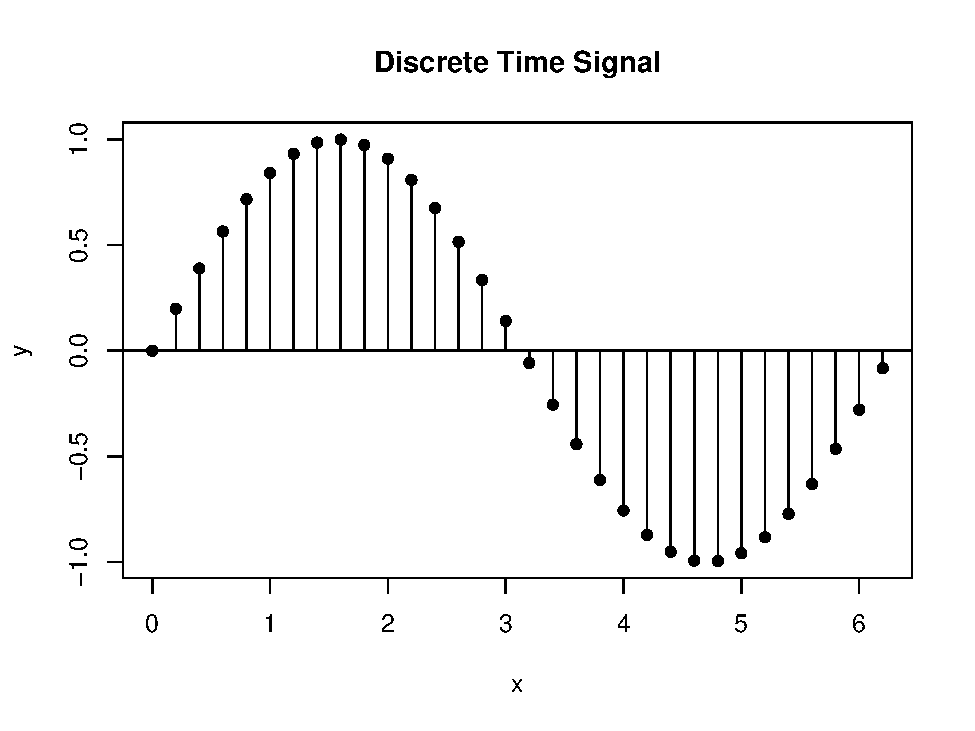
\includegraphics[width=0.8\linewidth]{stunning-chainsaw_files/figure-latex/nice-fig2-1} 

}

\caption{Here is a nice figure!}\label{fig:nice-fig2}
\end{figure}

\hypertarget{notation}{%
\subsection{Notation}\label{notation}}

Given an analog signal \(y(t)\), we can sample it at every \(T\) seconds. The resulting signal can be written as \(y(kT)\) where \(k\) now represents the sample step index.

If the signal is sampled at regular increments of time T, then T is also known as the Sample Period. The inverse of the sample period is the sample rate.

\begin{itemize}
\tightlist
\item
  Sample Period - \(T\) (seconds)
\item
  Sample Rate - \(1/T\) (1/seconds = Hertz), \(f_s\)
\end{itemize}

The notation \(y(kT)\) indicates a value of \(y{t}\) at \(t=kT\). The notation \(y[k]\) denotes a discrete time signal that is only defined only for \(k\) an integer. Written more succinctly: Parentheses indicate continuous time, brackets indicate discrete time.

It is important to reiterate that a discrete-time signal is only defined for \(k\) is an integer. A signal \(f[k]\) is defined when \(k\) is an integer; \(f[1.6]\) does not exist. However, the index for a discrete time signal may be positive or negative. A sequence, written as \({f[n]}\), may describe \(...,f[-2],f[-1],f[0],f[1],f[2],...\).

\hypertarget{discrete-amplitude-signal}{%
\subsection{Discrete-Amplitude Signal}\label{discrete-amplitude-signal}}

Most commonly, a discrete time signal is also a Discrete Amplitude signal. A discrete amplitude signal is a signal for which \(y[n]\) has only a finite possible amplitudes, in contrast to a continuous amplitude signal, for which the amplitude can assume any value \(\infty < y[n] < \infty\).

A discrete time, discrete amplitude signal is known as a Digital Signal. An example of a digital signal is the output of an analog-to-digital converter which converts a continuous time, continuous amplitude signal into a signal readable by a computer. The output of the analog-to-digital converter is represented by an eight bit binary number - which can only assume \(2^8 = 256\) unique values.

\hypertarget{fundamental-discrete-time-signals}{%
\section{Fundamental Discrete Time Signals\}}\label{fundamental-discrete-time-signals}}

\hypertarget{unit-step-function-and-unit-impulse-function}{%
\subsection{Unit Step Function and Unit Impulse Function}\label{unit-step-function-and-unit-impulse-function}}

The first two fundamental discrete time signals are the Unit Step Function and Unit Impulse Function.

The unit step function is defined by:
\begin{equation} \label{unitstepfunction}
u[k] = \begin{cases}
0, & k = -1, -2, \ldots \\
1, & k = 0, 1, 2, \ldots\\
\end{cases}
\end{equation}

The output of a unit step function \(f[k]\) is 0 for all integers of \(k\) less than 0, and is 1 for all integers of \(k\) equal to or greater than 0.

Similarly, the unit impulse function is defined by:
\begin{equation}
\delta[k] = \begin{cases}
1, k = 0 \\
0, otherwise\\
\end{cases}
\end{equation}

The output of a unit impulse function \(\delta[k]\) is 1 for \(k=0\) and is 0 for all other values of \(k\).

\hypertarget{time-shifting-time-scaling-time-reversal}{%
\subsection{Time Shifting, Time Scaling, Time Reversal}\label{time-shifting-time-scaling-time-reversal}}

Given a discrete time signal, it can be utilized with three time transformations: Discrete Time Shifting, Discrete Time Scaling and Discrete Time Reversal.

\textbf{Discrete Time Shift}
Given a signal \(y[k]\), the signal can be shifted along the time axis as \(y[k-2]\). This shifts the signal such that it starts 2 steps later - in otherwords, it delays the signal.

\hypertarget{crm-training}{%
\chapter{CRM Training}\label{crm-training}}

Attempt \#1

\begin{verbatim}
## PhantomJS not found. You can install it with webshot::install_phantomjs(). If it is installed, please make sure the phantomjs executable can be found via the PATH variable.
\end{verbatim}

\hypertarget{vo-training}{%
\chapter{VO Training}\label{vo-training}}

  \bibliography{book.bib,packages.bib}

\end{document}
